\documentclass[11pt]{report}
\usepackage[utf8]{inputenc}
\usepackage[T1]{fontenc}
\usepackage[francais]{babel}
\usepackage{amsmath}
\usepackage{graphicx}
\usepackage{listings}
\usepackage{booktabs}
\usepackage{subfig}

\usepackage{array}
\usepackage[dvipsnames]{xcolor}
\usepackage[colorinlistoftodos]{todonotes}
\usepackage{multirow}


\usepackage[top=3cm, bottom=3cm,left=2cm, right=2cm]{geometry}

\usepackage{hyperref}
\hypersetup{
    colorlinks,
    citecolor=black,
    filecolor=black,
    linkcolor=black,
    urlcolor=black
}

\begin{document}

%% Accents
\lstset{literate=
  {á}{{\'a}}1 {é}{{\'e}}1 {í}{{\'i}}1 {ó}{{\'o}}1 {ú}{{\'u}}1
  {Á}{{\'A}}1 {É}{{\'E}}1 {Í}{{\'I}}1 {Ó}{{\'O}}1 {Ú}{{\'U}}1
  {à}{{\`a}}1 {è}{{\`e}}1 {ì}{{\`i}}1 {ò}{{\`o}}1 {ù}{{\`u}}1
  {À}{{\`A}}1 {È}{{\'E}}1 {Ì}{{\`I}}1 {Ò}{{\`O}}1 {Ù}{{\`U}}1
  {ä}{{\"a}}1 {ë}{{\"e}}1 {ï}{{\"i}}1 {ö}{{\"o}}1 {ü}{{\"u}}1
  {Ä}{{\"A}}1 {Ë}{{\"E}}1 {Ï}{{\"I}}1 {Ö}{{\"O}}1 {Ü}{{\"U}}1
  {â}{{\^a}}1 {ê}{{\^e}}1 {î}{{\^i}}1 {ô}{{\^o}}1 {û}{{\^u}}1
  {Â}{{\^A}}1 {Ê}{{\^E}}1 {Î}{{\^I}}1 {Ô}{{\^O}}1 {Û}{{\^U}}1
  {œ}{{\oe}}1 {Œ}{{\OE}}1 {æ}{{\ae}}1 {Æ}{{\AE}}1 {ß}{{\ss}}1
  {ű}{{\H{u}}}1 {Ű}{{\H{U}}}1 {ő}{{\H{o}}}1 {Ő}{{\H{O}}}1
  {ç}{{\c c}}1 {Ç}{{\c C}}1 {ø}{{\o}}1 {å}{{\r a}}1 {Å}{{\r A}}1
  {€}{{\EUR}}1 {£}{{\pounds}}1
}
%% Couleur du code C
\lstdefinestyle{Cstyle}{language=C,
                basicstyle=\ttfamily,
                keywordstyle=\color{ForestGreen}\ttfamily,
                stringstyle=\color{orange}\ttfamily,
                commentstyle=\color{purple}\ttfamily,
                frame=single,
                numbers=left,                    % where to put the line-numbers; possible values are (none, left, right)
  			     numbersep=5pt,                   % how far the line-numbers are from the code
  				 numberstyle=\tiny\color{gray}, % the style that is used for the line-numbers
  				 rulecolor=\color{black},
                breaklines=true,
                stringstyle=\color{orange},
                morecomment=[l][\color{magenta}]{\#}
}

%% Page de titre
\begin{titlepage}
	
	\topskip0pt
	\newcommand{\HRule}{\rule{\linewidth}{0.5mm}}
	\center
	
	\vspace*{30pt}
	
	\textsc{\Large UFR Sciences et techniques\\ Université du Maine}\\[1.5cm]
	
	\Large RAPPORT DE PROJET\\[1.5cm]
	

	\vspace*{\fill}
	
	%% Titre du rapport de projet %%
	\HRule \\[0.4cm]
	{ \huge \bfseries RogueLike}\\
	\HRule \\[1.5cm]
	 
	 
	 \vspace{20pt}
	 
	{\large \today}\\[1cm]
	
	\vspace{12pt}
	
	\Large 
	
		Emeric \textsc{Mottier}\\
		Valentin \textsc{Pelloin}\\
		Titouan \textsc{Teyssier}\\
	
		\vspace{12pt}
		
		L2 Sciences pour l'ingénieur
		
	\vspace*{\fill}
	
\end{titlepage}

%% Partie sommaire
\tableofcontents

%% Partie introduction
\chapter{Introduction}

	Nous avons choisi le jeu \emph{Roguelike} car c'est un jeu que nous trouvons intéressant, puisqu'il est complet, et que c'est un jeu aux possibilités infinies :  il est toujours possible d'ajouter de nouvelles actions que le joueur pourra effectuer.
	
	\vspace{12pt}
	
	Notre jeu se déroule dans le bâtiment IC$_2$. Nous sommes un étudiant, nous partons du rez-de-chaussée, et nous devons aller chercher QUELQUE CHOSE tout en haut, pour le ramener. \\
	Nous devons cependant faire attention aux monstres : des L1, L2, L3, des masters, des doctorants, et certains fantômes : \textsc{Claude} et \textsc{Chappe}.\\
	Sur notre chemin, nous pouvons trouver quelques pièges : des flaques d'eau laissées par les femmes de ménages qui nous font glisser, des trous entre les étages qui nous font tomber d'un étage à un autre inférieur, ou des cartes à jouer qui nous sont jetées dessus par des L1.\\
	Durant notre parcours, nous devons aussi tenir compte de notre faim. Nous possédons une barre de vie, lorsqu'elle est à zéro, nous mourrons. Pour régénérer de la vie, il y a deux possibilités : ne plus avoir faim (en mangeant de la nourriture, attention, certaines sont empoisonnées), et des seringues de soin à s'injecter directement. Ces objets peuvent être consommés directement sur place quand le joueur le trouve, ou plus tard, en les gardant dans son inventaire.\\
	Enfin, lorsque le joueur apparait, il ne voit pas entièrement la carte, il doit la découvrir pour cela. Lorsque le joueur a trop faim, en plus de perdre de la vie, il s'évanouit : il se déplace plus difficilement, et perd connaissance de ce qu'il a découvert.
	
	\vspace{12pt}
	
	Pour le projet, nous devions au minimum effectuer un jeu qui génère des niveaux (ici, des étages dans notre bâtiment) aléatoires, avec une taille variant en fonction de l'étage où se trouve le joueur. Il était aussi demandé, en fonction de l'avancement du projet, d'ajouter des fonctionnalités supplémentaires : des armes, des monstres, des pièges, ou autres.
	
	\vspace{12pt}
	
	\begin{itemize}
	\item Le code source de notre projet, ainsi que les divers documents se trouvent à l'adresse :\\
		\hspace*{1cm} \href{https://github.com/TitouanT/rogueLike}{https://github.com/TitouanT/rogueLike}
	 \item La documentation de notre projet se trouve à l'adresse :\\
	 	\hspace*{1cm} \href{https://roguelike.vlntn.pw}{https://roguelike.vlntn.pw}
	 \item Notre répartition des tâches se trouve à l'adresse :\\
	 	\hspace*{1cm} \href{https://github.com/TitouanT/rogueLike/projects/1}{https://github.com/TitouanT/rogueLike/projects/1}
	\end{itemize}

%% Partie organisation
\chapter{Organisation}

Pour ce projet, nous avons dû nous organiser et trouver des outils afin de nous permettre de travailler à trois sur le code des uns des autres.

	\section{Répartition des tâches}

	Voici la répartition de tâches. Chaque personne a bien évidement aidé les autres en cas de problèmes.

\begin{table}[ht]
\centering
\caption{Notre répartition des tâches au sein du groupe}
\label{reparition}
\begin{tabular}{@{}lll@{}}
\toprule
\multicolumn{1}{c}{\textbf{Emeric}} & \multicolumn{1}{c}{\textbf{Valentin}} & \multicolumn{1}{c}{\textbf{Titouan}} \\
\midrule

- Gestion de la sauvegarde
& - Affichage
& - Definition des structures \\

\begin{tabular}[c]{@{}l@{}}- Gestion du changement \\ d'étages avec les escaliers\end{tabular}
& - Déplacement du joueur
& \begin{tabular}[c]{@{}l@{}}- Génération des niveaux (salles et \\ couloirs)\end{tabular} \\

\begin{tabular}[c]{@{}l@{}}- Ajout et comportement des \\ pièges\end{tabular}
& \begin{tabular}[c]{@{}l@{}}- Interactions (portes, nourriture, \\ kits de santé, ...)\end{tabular}
& - Ajout des portes entre les salles \\

& \begin{tabular}[c]{@{}l@{}}- Gestion de la régénération de\\ la vie\end{tabular}
& \begin{tabular}[c]{@{}l@{}}- Gestion des monstres (ajout, \\ déplacements, dégâts sur le \\ joueur, ...)\end{tabular} \\

& - Gestion de l'inventaire
& - Easter egg\\

\bottomrule
\end{tabular}
\end{table}

		\subsection{Pourquoi cette répartition}
		
		La répartition des tâches a été rapide, chacun a choisi ce qu'il voulait par exemple Titouan avait déjà fait de la génération de niveaux auparavant ce qui était un atout, Valentin voulait découvrir la bibliothèque ncurses et Emeric souhaitait gérer les sauvegardes.

	\section{Utilisation d'un gestionnaire de versions}
	
		Pour gérer les versions du projet nous avons utilisé Git et Github. Git pour toute la partie locale à chacune de nos machine. Quand nous codons, nous pouvons ainsi faire des versions du projet régulièrement et revenir en arrière si besoin. Github pour la mise en commun des modifications apportées, ce qui nous permet de travailler ensemble sans nécessairement coder en même temps ou au même endroit. Afin que chacun puisse librement ajouter ses modifications au projet, un seul dépôt Github a été créé et chaque membre de l'équipe a reçus le droit en écriture sur le dépôt.
	
	\section{Utilisation des projets Github}
	
		L'utilisation des projets de Github, découvert en conduite de projet, nous a permi de mettre tous nos objectifs sur le projet aussi bien que le code et le rapport. Nous avons créé une \emph{issue} pour chaque sujet, et nous avons aussi créé un milestone comme ça, nous pouvions être tenu au courant de l'avancée du projet et du travail des uns et des autres par rapport à la date butoire.
		Pour les objectifs du code, le lien du projet Github est le suivant : \href{https://github.com/TitouanT/rogueLike/projects/1}{ https://github.com/TitouanT/rogueLike/projects/1}. \\
		Et pour les objectifs du rapport :  \href{https://github.com/TitouanT/rogueLike/projects/2} {https://github.com/TitouanT/rogueLike/projects/2}.

	\section{Notre boîte à outils} 

		Notre projet a été réalisé en plusieurs modules différents, et l'un d'entre eux est notre boite à outil. Dedans se trouve de nombreuses fonctions qui nous sont utiles, mais qui ne sont pas pour autant liées à notre projet en particulier : des fonctions de comparaison d'intervalles, d'aléatoires, de caractères, de log d'erreurs, de fichiers, ...\\
		Nous avons aussi les fonctions essentielles pour l'accès à des listes et des files.

	\section{Doxygen, CUnit, GDB}\label{gdb}
	
		Durant la réalisation de notre projet, nous avons utilisé divers outils d'aide à la programmation et au débogage. 
		
		\vspace{12pt}		
		
		La première chose que nous avons mis en place est la documentation à l'aide de \emph{Doxygen}. C'est un programme qui génère une documentation automatiquement, en fonction des fichiers d'en-têtes et sources. La documentation peut être générée de plusieurs formats, nous avons choisi au format HTML car il est plus facile de s'en servir. Celle-ci est sur internet, à l'adresse suivante : \url{https://roguelike.vlntn.pw/}. Elle se met à jour automatiquement en fonction de notre code (via un webhook mis en place sur Github).
		
		\vspace{12pt}
		
		Ensuite, nous avons utilisé \emph{CUnit}, un \emph{framework} de tests unitaires pour le C. Toutes nos fonctions de notre boîte à outil ont été testés, avec des assertions que nous jugeons pertinentes (sur des valeurs qui pourraient poser problème dans certaines fonctions, comme des valeurs nulles, négatives, sur des fichiers inexistants, ...).
		
		\vspace{12pt}
		
		Enfin, lorsque nous avions certains bogues que nous n'arrivions pas à résoudre, nous avons utilisé le logiciel de débogage \emph{GDB} (\emph{GNU DeBugger}). Nous n'avions pas réussi à le faire fonctionner dès le début, car nous utilisons la libraire d'affichage \emph{ncurses}\footnote{Voir la section \hyperref[ncurses]{interactions et déplacements, page \getpagerefnumber{ncurses}}.}, qui utilise déjà le terminal pour afficher notre jeu. En le combinant avec \emph{GDB}, le terminal n'était plus utilisable.\\
		La solution à été d'utiliser deux téléscripteurs (\textsc{TTY}) différents : un pour le jeu, et un pour le débogueur.\\
		Dans l'annexe, vous pouvez retrouver 3 exemples de cas où nous nous sommes servis du débogueur.

%% Partie analyse et conception
\chapter{Analyse et Conception}

	Avant de commencer à programmer notre jeu, nous nous sommes concertés autour d'un même fichier pour mettre en commun nos idées à propos du jeu. Notre jeu étant très libre dans son fonctionnement, c'était une étape cruciale.\\
	Nous n'avons pas néanmoins réalisé un cahier des charges <<conventionnel>>, car nous trouvions que c'est quelque chose de figé, et qu'au fur et à mesure de l'avancement du projet, celui-ci n'évoluait pas en fonction de ce nous voulions. Nous avons donc réalisé un document listant tous les points importants de notre projet, et quelques détails importants. Toutes les autres choses ont été définies entre nous, lors de la réalisation du projet.

	\section{Notre cahier des charges}


	Notre \emph{rogueLike} prend place dans le bâtiment IC$^2$. Le joueur démarre le jeu au premier étage. Il doit se rendre tout en haut, aller chercher l'objet, puis revenir en bas.\\
	Chaque étage de ce bâtiment est généré aléatoirement, il doit comporter des pièces et des couloirs. Entre ceux-ci, peut se trouver des portes, ou juste un trou. Les portes sont aléatoirement ouvertes ou fermées, et le joueur peut essayer de les ouvrir manuellement (il a une probabilité de ne pas réussir). Le nombre de pièces par étage est défini en fonction de l'étage : les étages supérieurs sont plus compliqués car ils possèdent plus de pièces. Pour changer d'étages, le joueur doit emprunter des escaliers (un escalier pour monter, et un pour descendre par étage, ceux-ci ne peuvent pas se trouver dans la même pièce).\\
	Lorsque le joueur apparait, il ne voit que la pièces où il se situe. Dans les couloirs, lorsqu'il progresse, les zones s'éclairent petit à petit, en revanche, dans dès qu'il entre dans une pièce, celle-ci s'éclaire entièrement.\\
	Le joueur possède un certain nombre de point de vie (défini à 10) au maximum, lorsque celle-ci est à 0, il meurt. Au fur et à mesure de ses déplacements, il perd de la nourriture (une barre allant de 0 à 100). Lorsqu'il a trop faim (nourriture inférieure à 10), il ne se déplace plus correctement, il perd certaines zones de sa mémoire de la carte (elle ne sont plus éclairées), et il perd de la vie. Le joueur peut trouver de la nourriture aléatoirement par terre (un total de 2 objets de nourriture par pièce, par étage), tout comme il peut trouver des soins de santé pour lui faire régénérer sa vie. L'autre façon de re-gagner de la vie est de manger, ainsi certains point de nourritures seront utilisées pour la vie.\\
	Lorsque le joueur mange de la nourriture, il a une faible probabilité de chance que celle-ci était empoisonnée. Le joueur perd de la vie à chaque déplacement lorsqu'il est empoisonné. Pour ne plus l'être, il doit soit attendre quelques déplacements de ne plus l'être, soit consommer un kit de santé.\\
	Durant son chemin dans le bâtiment, le joueur peut se faire avoir par des pièges. Ceux-ci peuvent, au choix, enlever de la vie, nous faire glisser à travers la pièce, ou nous faire tomber d'un ou plusieurs étages (une chance sur 3 pour chaque).\\
	Les objets tels que la nourriture, les soins de santé, ou les pièges peuvent être récupérés par le joueur dans son inventaire, pour les déposer ou les utiliser plus tard. L'inventaire du joueur possède 5 \emph{slots}, et il ne peut y déposer qu'un seul objet par \emph{slot}.\\
	Des monstres se trouvent dans le jeu, ceux-ci nous attaquent, en se rapprochant de nous. Nous pouvons aussi les attaquer. Ils possèdent, tout comme nous, une agilité, qui est plus importante pour un monstre évolué. Cette agilité permet de faire plus de dégâts au combat, et de moins en subir. Ces monstres doivent avoir une mini-intelligence artificielle pour qu'ils puissent se déplacer de façon similaire à ce que un véritable joueur pourrait faire.
	
	\vspace{12pt}

	A tout moment, l'utilisateur peut sauvegarder sa partie sur l'un des trois emplacements de sauvegarde prévus. Il peut aussi quitter le jeu à n'importe quelle étape. Au lancement, l'utilisateur doit avoir un écran lui indiquant les sauvegardes, il peut en charger une, ou en supprimer une. Si il lance le jeu sur un emplacement vide, une nouvelle partie est alors crée.\\
	A la fin du jeu, lorsque le joueur perd, ou gagne, il se retrouve sur l'écran initial des sauvegardes.\\
	Au lancement du jeu, un texte explicatif avec l'objectif de celui-ci doit être affiché. Le jeu est décomposé en trois parties :
	\begin{itemize}
	\item la zone de jeu
	\item la zone de \emph{logs}, où se trouve des informations sur ce que le joueur peut effectuer
	\item la zone de statistiques, qui indique toutes les propriétés du joueur : étage, vie, faim, nombre de déplacements, si il est empoisonné, si il a trouvé l'objet, ...
	\end{itemize}
	
	
	\section{Comment jouer ?}
		\begin{itemize}
			\item{Lancement du jeu : \\}
				Pour commencer à jouer, vous devez télécharger le jeu à partir de l'adresse suivante : \href{https://github.com/TitouanT/rogueLike/} {rogueLike}; avec la commande suivante : \texttt{git clone git@github.com:TitouanT/rogueLike.git}
				Vous faîtes : \texttt{cd rogueLike}. \\
				Puis vous compilez grâce au makefile : \texttt{make install}. \\
				Le jeu commence dès que vous faîtes : \texttt{./rogueLike}.	
			\item{Les déplacement : \\}
				Nous pouvons gérer nos déplacements sur la carte grâce aux flèches de direction. 
			\item{Interactions avec des objets : \\}	
				Les interactions avec un objet (seringues de soins, nourriture, escalier) se font avec la touche \texttt{entrée}.
			\item{Ouvrir et fermer une porte :\\}	
				Si vous souhaitez ouvrir une porte, déplacez-vous devant la porte, appuyer sur la touche \texttt{o} et marqué la direction de la porte avec les flèches de direction.
				Mais pour fermer, c'est le même principe que pour ouvrir une porte sauf que la touche est \texttt{c} au lieu de \texttt{o}.
			\item{Gestion de l'inventaire : \\}
				Pour voir votre inventaire, vous devez appuyer sur la touche \texttt{i}. Pour prendre un objet (seringues de soins, nourriture), vous devez appuyez sur la touche \texttt{g} mais pour poser votre inventaire, vous devez appuyez sur la touche <<d>> et indiquer la case se trouve l'objet.
			\item{Sauvegarder sa partie :\\}
				Vous pouvez sauvegarder la partie à tout moment avec la touche \texttt{s}, cette manœuvre n'arrêtera pas votre expérience de jeu.
			\item{Combattre un monstre :\\}
				Pour combattre un monstre, utilisez les flèches de direction et déplacez vous sur le monstre jusqu'à ce qu'il meurt (disparaisse).		
		\end{itemize}
		Ces commandes sont accessibles dans le jeu en appuyant sur la touche \texttt{?}.
		Certains commandes sont encore à découvrir comme se déplacer en diagonale pour échapper à des monstres ou des codes de triches peuvent être utiliser grâce à la touche \texttt{\_}, pour les voir faîtes \texttt{\_} et taper \texttt{help} pour avoir la liste.
		
%% Partie codage
\chapter{Codage, méthode et outil}

ici mettre un petit mot

	\section{Structures et énumérations}
	
	Nous avons utilisé un certain nombre de structure et d'énumération pour modéliser le rogueLike.
	
		\subsection{Une case de la carte}
	
		La structure la plus importante est celle qui représente une case de la carte. Cette structure contient un champ qui définit sont type, un autre qui défini son état ainsi qu'un tableau listant les objet présent sur la case et deux entiers pour savoir si le joueur a découvert cette case et pour connaitre le nombre d'objets présent.
	
		Le type est une énumération des différents type de case possible: un vide, un mur, un encadrement de porte, une pièce ou un couloir.
	
		L'état est une énumération utilisé pour les encadrements de portes afin de savoir si il y a une porte, et si elle est ouverte ou fermée. L'état est aussi utilisé pour les pièces afin de savoir si il y a de la lumière ou non dans la pièce.
	
		Un objet est décrit par une structure qui est composé d'un type et d'un entier pour savoir si l'objet a été découvert par le joueur. Le type d'un objet est lui décrit par une énumération et définit les escaliers ascendants et descendants, la nourriture, les kits de santé et les pièges.
		
		\subsection{Les être vivants}
		
		Le joueur contrôle un personnage que l'on représente à l'aide d'une structure. Elle permet d'enregistrer son nom, sa position (ligne, colonne et niveau), ses points de vie et d'attaque, son agilité, son expérience, son appétit, sa santé, le nombre de mouvement effectué, un booléen pour savoir si il a trouvé le QUELQUE CHOSE ainsi qu'un tableau d'objet qui représente son inventaire.
		
		Les monstres ont eux aussi une structure qui enregistre leur nom, leur types, leur position (ligne, colonne et niveau), leur points de vie et d'attaque, leur champ de vision, leur agilité et quelque champs supplémentaire qui est utilisé comme mémoire pour leur IA. Les différents types de monstres sont L1, L2, L3, master, doctorant et fantôme.
		
		\subsection{Et le reste}
		
		La représentation en matrice des niveau n'étant pas dans tous les cas la plus efficace, nous avons créé une structure de niveau qui contient un tableau de pièces et le nombre de pièces que contient l'étage.
		
		Une pièce est elle-même représentée par une structure qui contient la position de son angle supérieur gauche (ligne et colonne) ainsi que ses dimensions (largeur et hauteur).
		
		Quelque fois, nous avons besoin de manipuler des position (ligne, colonne). Nous avons donc créé une structure de position qui contient une ligne et une colonne. 
		
	\section{Séparation du code en modules}
	
	Afin d'avoir un code source clair et maintenable, nous l'avons séparé en plusieurs modules. Nous avons un module dédié pour:
	\begin{itemize}
		\item les affichages,
		\item les interactions (interprète les commandes du joueur),
		\item les lectures/écritures dans des fichiers,
		\item la boîte à outils,
		\item la génération des niveaux,
		\item et la prise en charge des monstres.
	\end{itemize}
	
	
	\section{Détail des principales fonctionnalités du jeu}

	Voici un descriptif des principales fonctionnalités du programme, et de leur mise en place dans notre projet.
	
		\subsection{La génération des niveaux}
		
		La génération d'un niveau ce fait en quelques étapes:
		\begin{enumerate}
			\item Le choix du nombre de pièce à placer en fonction de l'étage qu'il représente (de 0 à 5).
			\item Le placement des pièces sur la carte.
			\item La création des couloirs pour lier les pièces.
			\item Le placement des objets (nourriture, escaliers, pièges).
		\end{enumerate}
		
			\subsubsection{Placement des pièces}
			
			Pour placer les pièces, on les places les unes après les autres. Pour chaque pièces, nous commençons par lui donner une position (la position de son angle supérieur gauche). Ensuite nous lui choisissons une dimension (hauteur, largeur) afin qu'elle entre la plus petite et la plus grande pièce possible.
			Pour finir, nous vérifions qu'elle n'est pas en collision avec une autre pièce.
			Dans le cas ou elle l'est, on recommence (pas plus de 100 fois).
			
			\subsubsection{Création des couloirs}
			
			Le but est de créer un réseau de pièces ou aucune pièce ou groupe de pièces ne soit isolé des autres.
			Pour cela nous connectons les pièces les unes après les autres dans leur ordre de création.
			L'algorithme qui créé les liens commence par initialiser la première pièces simplement en y ouvrant une porte.
			Ensuite, pour chaque pièces il procède ainsi:
			\begin{itemize}
				\item Création d'une ouverture dans la pièce.
				\item Création d'un couloir entre cette ouverture et la case de type couloir ou encadrement de porte la plus proche à l'aide d'un algorithme de recherche de chemin.
			\end{itemize}
		
		\subsection{Les lectures et les écritures dans des fichiers}
		
		Nous gérons des sauvegardes sur plusieurs fichiers:
		\begin{itemize}
			\item Des fichiers comportant les paramètres l'ensemble des niveaux, soit un fichier texte pour un niveau ; nommé lvl.txt avec lvl variant selon le niveau.
			\item Un fichier texte comportant les donnes sur les monstres présents dans la partie ; nommé : monster.txt.
			\item un fichier comportant les données de chaque pièce ; nommé : lvlData.txt.
			\item un fichier comportant les données du personnage ; nommé : position.txt.
		\end{itemize} 
		\subsubsection{Les écritures :}
		Les niveaux sont sauvegardés lorsque du lancement d'une nouvelle partie, un changement de niveau, lorsque le joueur demande de sauvegarder. Les monstres sont sauvegardés lors de la création d'une nouvelle partie et la sauvegarde demandéé par le joueur. Les données de chaque pièce sont sauvegardées que lors d'une nouvelle partie. Quant aux données du personnage, elles sont sauvegardées que lorsque le joueur veut sauvegarder, l'apparition de cette sauvegarde montre qu'une partie est sauvegardée : si ce fichier n'existe pas lors du relancement du jeu, le joueur n'aura pas accès à ses anciennes données.

		\subsubsection{Les lectures :}
		Les niveaux sont lus si le joueur veut charger une partie sauvegardée, un changement de niveau. Les monstres sont lus lors du chargement d'une partie existante comme les données sur le joueur et les données des pièces.

		\subsection{Les interactions et déplacements}\label{ncurses}

		
			Notre jeu devait se jouer de façon simple, le joueur devait pouvoir déplacer son personnage d'un simple appui sur une touche. L'utilisation de simples \texttt{scanf()} pour récupérer l'appui sur une touche aurait été difficile à gérer, car ces fonctions sont exécutées uniquement lorsque la personne appuie sur la touche \textit{entrée}. Pour palier ce problème, nous avons utilisé la libraire \emph{ncurses}, qui est une \textsc{TUI}, une interface utilisateur par terminal. Celle-ci nous permet, entre autres, de récupérer les touches (ou combinaisons de touches) que l'utilisateur effectue sans avoir à attendre qu'il appuie sur entrée.
			
			
		\subsection{L'affichage}
		
		L'affichage s'est aussi faite à l'aide de la libraire \emph{ncurses}, car elle propose des fonctions de création de fenêtres virtuelles, et d'écriture directement sur celles-ci. Nous avons séparé notre jeu en trois zones, qui sont en réalité des fenêtres. Pour l'écran de chargement et de fin de partie (en cas de perte ou de victoire), des messages ASCII sont affichés, ces messages proviennent en réalité de fichiers textes, qui sont lus par le programme et affichés au centre de l'écran. L'écran de sélection quant à lui nous permet de visualiser facilement, avec des couleurs, les parties.
		
		\vspace{12pt}
		
		Lorsque le joueur découvre de nouveaux endroits dans les couloirs, l'état de visibilité des cases l'entourant change. Pour le pièces, puisque celles-ci doivent s'allumer entièrement, on vérifie si le joueur se trouve dans une pièce. Dans ce cas, on cherche la taille de la pièce où se trouve le joueur, puis on affiche chaque case de celle-ci.\\
		Au moment d'afficher la carte, on n'oublie pas d'afficher les cases uniquement si elles sont visibles.
		
		\subsection{Les monstres}
		
		Le nombre de monstre dans une partie est choisi aléatoirement entre deux bornes définies en constantes.\\
		Les monstres sont équitablement répartis entre les étages proportionnellement au nombres de pièces qu'ils contiennent. Chaque étages a une proportion différentes de chaque monstres, plus l'étage est haut, plus les types de monstres présents sont difficiles à battre.\\
		Pour animer les monstres, nous marquons toutes les cases de la matrice accessible par le joueur avec la distance de celle-ci par rapport au joueur. Ensuite chaque monstre fait un mouvement en direction du joueur si le joueur est dans son champ de vision. Sinon, ils ne bougent pas.\\
		Nous faisons attention à ce que les monstres n'aillent pas sur le joueur et si le joueur est à porté alors ils l'attaquent. Si le joueur fait un déplacement vers une case ou se trouve un monstre alors le joueur ne bouge pas et attaque. Ainsi, il n'y a jamais deux êtres vivants sur la même case.
		
		Les fantômes sont particuliers car :
		\begin{itemize}
			\item ils ne visent jamais le joueur,
			\item ils peuvent se déplacer partout sur la carte,
			\item ils ont un halo lumineux autour d'eux, permettant au joueur d'apercevoir des zones qu'il n'a pas encore découvertes.
		\end{itemize}
		
		\subsection{La nourriture et la vie}
		
		A la génération des niveaux, nous sélectionnons des endroits libres (mais aléatoires) sur la carte, dans des pièces, pour y placer des objets de nourriture, et des objets de santé. Le nombre de ces objets trouvable dans le niveau est défini en fonction du nombre de pièces de celui-ci. \\ Lorsque le joueur se trouve sur un de ses objets, et qu'il effectue l'action pour s'en servir, sa nourriture ou sa vie est mise à jour. Ensuite, à chaque tour, on vérifie si le joueur possède plus de 90\% de nourriture. Dans se cas, il possède une chance sur trois d'augmenter sa vie (et de diminuer sa nourriture). Si il ne possédait pas 90\% de nourriture, alors il possède 1\% de chance d'augmenter sa vie.\\
		Lorsque le joueur ne possède plus de vie, il possède 75\% de ne pas réussir à se déplacer. Pour l'évanouissement, une position est choisie aléatoirement, puis deux longueurs, entre deux bornes. Le rectangle formé par ces données est ensuite passé en non-visible.
		
		\subsection{L'inventaire du joueur}

		L'inventaire du joueur est en réalité un tableau du même type que les objets de notre carte. Ainsi, lorsqu'on souhaite ajouter un objet à l'inventaire du joueur, il suffit de prendre l'objet, et le mettre dans l'inventaire, à une case disponible. Lorsque le joueur souhaite poser un objet, il lui est simplement demandé un indice (correspondant à l'indice du tableau de son inventaire), et l'objet présent à cet endroit, si il existe, est posé au pied du joueur. Dans chaque cas, il faut faire attention que le joueur se trouve sur une case contenant aucun objet.

%% Partie conclusion
\chapter{Résultat et conclusion}

	Les objectifs de l'énoncé ont été atteint, 
	
	\section{Améliorations possibles}
	
	Il aurait été possible d'améliorer notre projet en ajoutant des sons dans le jeu. On aurait aussi pu créer un didacticiel. \\
	Le but aurait été d'ajouter un fond sonore dans le jeu et des sons lorsqu'un monstre attaque, ou est proche du joueur. Pleins de possibilités pourraient s'offrir à nous lorsque que nous trouverons un moyen de lire une bande son (avec un réglage pour de ne pas mettre de son pour ceux qui le souhaitent). \\
	Un didacticiel serait aussi intéressant pour apprendre au joueur à jouer.\\
	Un système de classe aurait pu être intéressant, au début, nous aurions pu choisir d'être un humain, un elfe, un nain, ou autre, avec des caractéristiques différentes (vie, vitesse, attaque, résistance, faim moyenne du joueur, ...).\\
	Enfin, un développement du système d'expérience aurait rendu notre jeu plus jouable : lorsqu'un joueur tue un monstre, son expérience augmente, et plus son expérience est élevée plus il tue facilement d'autres monstres.
	
	\section{Apport personnel du projet}
	
	Voici l'apport personnel du projet, pour chaque membre du groupe :
	
	\begin{description}
	\item[Valentin :] Dans mon cas, le projet m'a permis de découvrir une librairie qui est \emph{ncurses}. Cette librairie est pratique car elle est plus simple à manipuler que la \emph{SDL} par exemple. De plus, le \emph{Rogue} est un jeu qui se joue généralement dans un terminal, \emph{ncruses} s'adapte parfaitement à notre projet. Le projet m'a aussi permis de me rendre compte à quel point la gestion peut être difficile, et conflictuelle. Il faut savoir gérer le temps, la répartition des taches. Il faut aussi savoir adapter le projet en fonction de son avancement, pour ne pas stagner. Enfin, notre projet étant assez libre dans son fonctionnement, beaucoup de fonctionnalités autour de celui-ci sont des détails, que chaque personne peut voir dans une manière différente que les autres. 
	\item[Emeric :] Pour moi, ce projet a été une façon de voir ce que le travail de groupe peut avoir comme influence sur un projet d'informatique. Nous étions parti pour faire la génération des niveaux, l'affichage, les déplacements et la sauvegarde sur deux semaines et au bout d'une semaine, nous avions presque fait tous ces objectifs. Voir un de ses collègue avancer, ça donne envie d'avancer autant que lui et nous arrivons à un effet boule de neige.
	\item[Titouan :] Ce projet as été très intéressant pour deux choses. Premierement, travaillé en équipe de trois est, je pense, une configuration des plus conflictuelle. Il nous à donc fallu souvent faire des compromis pour que chacun puisse s'approprier le jeu. L'écriture du rogueLike a donc été une première expérience de travail en équipe. Secondement, la taille du rogueLike étant de loin la plus importante de tous mes précédents programmes, c'est pour ce projet que j'ai réalisé à quel point la programmation modulaire est efficace, claire et maintenable.
	\end{description}

\chapter*{Annexe}

	\section*{Cas d'utilisation du débogueur \emph{GDB}}
	
		Parfois, nous n'arrivons pas à trouver la cause de certains bugs, qui étaient finalement très simple. Pour cela, nous avons utilisé l'outil \emph{GDB}, comme mentionné dans \hyperref[gdb]{la partie sur les outils, page \getpagerefnumber{gdb}}. Afin de l'utiliser avec \emph{ncurses}, voici la marche à suivre :
		
		\begin{enumerate}
		\item Ouvrir deux terminaux, un qui servira d'interface pour \emph{GDB}, un autre, suffisamment grand pour notre jeu.
		\item Sur le terminal du jeu, tapez la commande \texttt{tty} afin de connaître le nom du \emph{TTY} de celui-ci. Tapez ensuite la commande \texttt{sleep 10000000} afin de dire au terminal d'attendre longtemps avant de faire une autre action.
		\item Sur le terminal du débogueur, tapez le commande \texttt{gdb rogueLike} afin de lance \emph{GDB} sur notre programme.
		\item Une fois dans \emph{GDB}, tapez \texttt{tty <nom du TTY>} avec \texttt{<nom du TTY>} celui trouvé à l'étape 2. Il est généralement de la forme \texttt{/dev/ttys000}.
		\item Vous pouvez maintenant utiliser \emph{GDB}.
		\end{enumerate}


	\subsection*{Des monstres qui passent à travers les portes ...}
		Il arrivait parfois que des monstres passent à travers des portes fermées. Nous avons lancé \emph{GDB}, et nous nous sommes rendu compte que la fonction qui testait si un monstre pouvait marcher sur une case était inversée dans le cas des portes :

			\begin{figure}[ht]
			    \centering
			    \subfloat[Porte fermée, monstre à l'intérieur]{{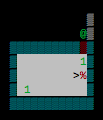
\includegraphics[width=2cm]{images/monsters_through_doors/explication_1.png}}}
			    \qquad
			    \subfloat[Il a réussi à aller sur la porte]{{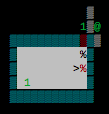
\includegraphics[width=2cm]{images/monsters_through_doors/explication_2.png} }}%
			    \caption{Explication du beug}%
			\end{figure}

	\newpage

			\begin{figure}[ht]
			    \centering
			    \subfloat[Lancement de \emph{GDB}]{{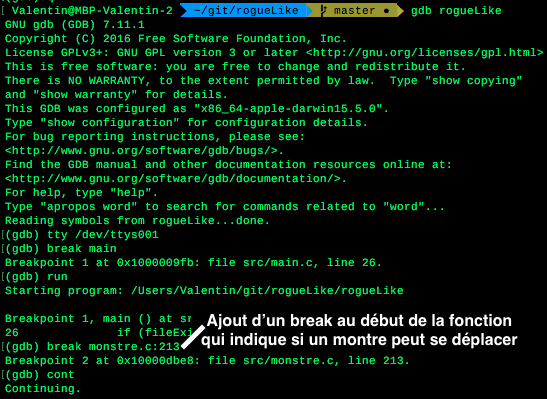
\includegraphics[width=10cm]{images/monsters_through_doors/dbt_gdb.png}}}
			    \qquad
			    \subfloat[Erreur trouvée]{{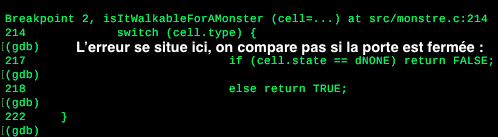
\includegraphics[width=10cm]{images/monsters_through_doors/erreur.png} }}%
			    \caption{Résolution du beug}%
			\end{figure}
		
		\newpage
	\subsection*{Nourriture qui baisse trop vite ...}
		Lors de l'ajout de la nourriture, nous nous sommes vite rendu compte qu'elle diminuait à chaque tour, malgré la probabilité de 70\% qu'elle ne diminue pas. Nous avons lancé \emph{GDB}, nous avons tout d'abord vérifié que la nourriture était bien prise en compte dans les caractéristiques du joueur. Ensuite, en regardant de plus près la fonction qui gère la faim, nous avons pu tester manuellement les conditions pour la diminution de la nourriture. Nous nous sommes rendu compte que le \emph{OU} de la condition était incorrect, et aurait du être un \emph{ET}.
		
			\begin{figure}[ht]
			    \centering
			    \subfloat[La nourriture est prise en compte]{{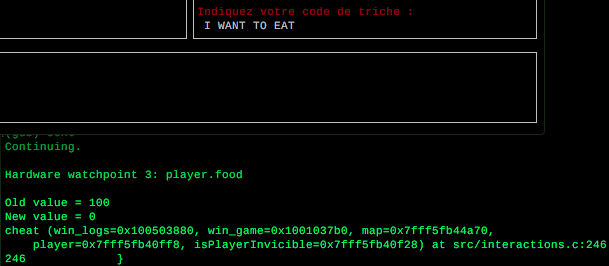
\includegraphics[width=8cm]{images/bouffe_qui_baisse_pas/la_bouffe_est_bien_geree.png}}}
			    \qquad
			    \subfloat[Les conditions \emph{OU} sont incorrectes]{{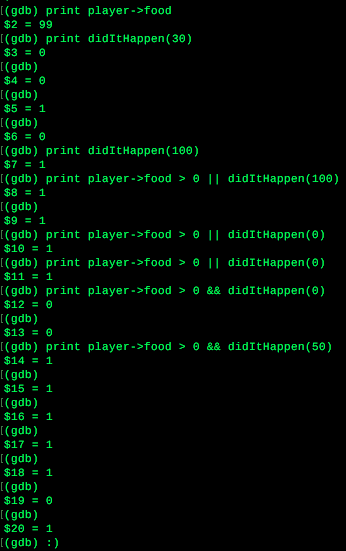
\includegraphics[width=5cm]{images/bouffe_qui_baisse_pas/ou_ou_et_that_is_the_question.png} }}%
			    \caption{Résolution de la nourriture qui baisse vite}%
			\end{figure}
	
	\subsection*{Pièges qui apparaissent dans les couloirs ?}
	
		Le problème qui nous a pris le plus de temps à résoudre fut celui qui faisait apparaître des pièges dans les couloirs de façon très aléatoire. Nous n'arrivions jamais à reproduire deux fois de suite l'erreur, même sur une même partie au même endroit. Nous pensions au début que cela venait de la génération des pièges, mais celle-ci était correcte. Après l'utilisation du débogueur, nous nous sommes rendu compte que la condition qui testait si le joueur se trouvait sur un piège n'était pas complète. En effet, nous testions si l'objet se trouvant à la case du joueur était un piège, sans jamais vérifier qu'un objet s'y trouvait. Or la liste des objets n'est pas remise à zéro lorsqu'on charge un nouvel étage. Donc un piège d'un autre étage peut avoir de l'effet sur un autre n'en contenant pas.




			\begin{figure}[ht]
				\centering
				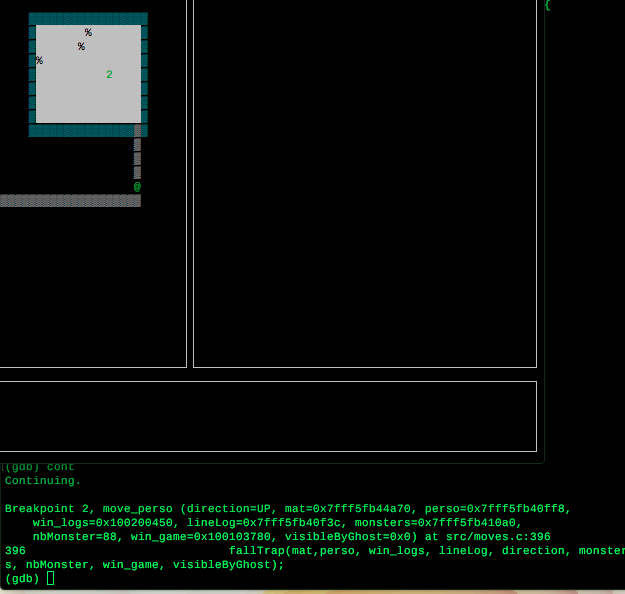
\includegraphics[width=8cm]{images/pieges_dans_les_couloirs/wtf.png}
				\caption{On tombe dans un piège en étant dans un couloir}
			\end{figure}

			\begin{figure}[ht]
			    \centering
			    \subfloat[Pas de piège où nous sommes]{{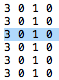
\includegraphics[width=3cm]{images/pieges_dans_les_couloirs/y_a_pas_de_piege.png}}}
			    \qquad
			    \subfloat[Condition incomplète]{{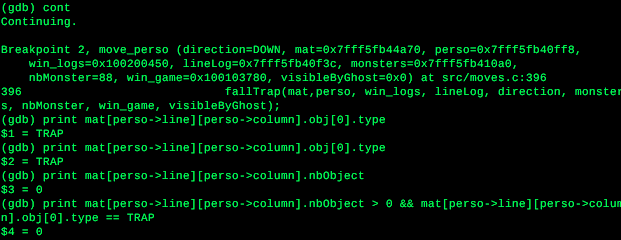
\includegraphics[width=10cm]{images/pieges_dans_les_couloirs/on_teste_pas_le_nb_obj.png} }}%
			    \caption{Résolution de la nourriture qui baisse vite}%
			\end{figure}		
		
\end{document}